\chapter{Remaining Useful Life Prediction}
\label{chap: rul}

In this chapter, we propose a framework for predicting RUL of fatigue damaged samples based on the ultrasonic testing. The framework has two parts: \begin{enumerate*}[label=\itshape\alph*\upshape)]
    \item an ML classification task and
    \item an RUL inference procedure based on an S-N curve.
\end{enumerate*}  First, ultrasonic signals are fed into ML classifiers to predict the loading condition and the percentage of fatigue life that a sample has gone through. Second, we estimate RUL from an S-N curve with the predicted loading condition and percentage of fatigue life.

\section{Problem formulation}
\label{sec: rul prob formulation}
Given the goal of predicting the RUL of EoL products, we need to formulate this as an ML problem first. In this section, We discuss possible formulations by considering the characteristics of the fatigue dataset and the impact on the ML system.

\subsection{Dataset}
In this RUL prediction task, the dataset is constructed on the ultrasonic measurements from the interrupted fatigue testing specimens in Table \ref{table: interrupted specimens}. There are 15 specimens and each of these were measured at 9 locations alongside 3 repeated measurements, producing 405 observations in total. Notice that we treat one measurement location in one specimen as a sample in the model training and validation procedure with LOGOCV, as described in Section \ref{sec: model train and val}. Besides, each specimen is tested by a combination of fatigue condition from 4 loading amplitudes and 3 fatigue levels (the percentage of fatigue life), which forms the labels of a specimen.

\subsection{Target variables}
RUL is intuitively translated by the percentage of fatigue life that a sample has gone through. Normally, the percentage of fatigue life as a continuous target variable is treated as a regression task. However, since we only have 3 different percentage of fatigue life in the dataset, which is not ideal for regression modeling, we decided to view the percentage of fatigue life as a discrete variable and the problem becomes a classification task.

Loading amplitude is another target variable to be considered because loading condition affects the mechanism of fatigue damage in a material. For instance, at 33\% fatigue life, a sample experienced 11.7 kN loading and a sample experienced 14.7 kN loading could exist different fatigue damages. Hence, we place a label that is a combination of loading amplitude and the percentage of fatigue life on each sample. Table \ref{table: rul dataset} presents the labeled RUL prediction dataset.

\begin{table}[tb]
    \centering
    \caption{Summary of the RUL prediction dataset}
    \label{table: rul dataset}
    \begin{tabularx}{\textwidth}{
      >{\centering\arraybackslash\hsize=0.5\hsize}X|
      >{\centering\arraybackslash\hsize=0.6\hsize}X|
      >{\centering\arraybackslash\hsize=0.6\hsize}X|
      >{\centering\arraybackslash}X
    }\hline
      Specimen ID & Number of Measurement Locations & Number of Repeated Measurements & Label (amplitude, percentage of fatigue life) \\
      \hline
          1&\multirow{15}{*}{9}&\multirow{15}{*}{3}&\multirow{2}{*}{Class 1 (11.7 kN, 33\%)}\\
          2& & & \\
          \cline{1-1}\cline{4-4}
          3& & &\multirow{2}{*}{Class 2 (11.7 kN, 67\%)}\\
          4& & & \\
          \cline{1-1}\cline{4-4}
          5& & &\multirow{2}{*}{Class 3 (12.7 kN, 33\%)}\\
          6& & & \\
          \cline{1-1}\cline{4-4}
          7& & &\multirow{2}{*}{Class 4 (12.7 kN, 67\%)}\\
          8& & & \\
          \cline{1-1}\cline{4-4}
          9& & &\multirow{2}{*}{Class 5 (14.7 kN, 33\%)}\\
          10& & & \\
          \cline{1-1}\cline{4-4}
          11& & &\multirow{2}{*}{Class 6 (14.7 kN, 67\%)}\\
          12& & & \\
          \cline{1-1}\cline{4-4}
          13& & &\multirow{3}{*}{Class 0 (0 kN, 0\%)}\\
          14& & & \\
          15& & & \\\hline
    \end{tabularx}
\end{table}

\section{Design of classifiers}
\label{sec: design of classifiers}
In this section, classifiers are designed for predicting the loading condition (amplitude) and the percentage of fatigue life that a sample had experienced. Several classifiers are developed and the performance of each of those methods is evaluated based on the model development procedure in Chapter \ref{chap: model}.

\subsection{Multi-class classifier}
A multi-class classifier is trained to classify a sample into 1 of the 7 classes. Figure XXX shows the inference process of a multi-class classifier. In multi-class problems, the classes are mutually exclusive. For example, class 1 and class 3 have nothing in common. However, despite we claimed that various loading conditions result in different fatigue behaviors in material, some similarities still exist, e.g., at 33\% fatigue life, samples undergone 11.7 kN and samples undergone 12.7 kN are expected to be at a similar damage level. This idea can be applied to the commonality in samples at different percentages of fatigue life as well. With the assumption of mutual exclusivity, multi-class formulation cannot capture these characteristics of the fatigue data.

\subsection{Multi-output classifier}
\label{subsec: multi-output classifier}
On the other hand, multi-output classification is capable of dealing with mutually non-exclusive classes by predicting the loading amplitude and percentage of fatigue life separately. A multi-output classifier outputs multiple labels, where each label is considered a multi-class classification problem. In this design, we build one classifier for predicting the loading amplitude from input signals; another one for classifying a signal into one of the percentages of fatigue life. Then, the two predicted labels are combined based on a rule-based algorithm to output a class label that is consistent with the label in the dataset, as depicted in Figure XXX. We call these two classifiers a loading amplitude classifier (LAC) and a fatigue cycle classifier (FCC), respectively. Each of the two classifiers are trained separately with the same model development procedure but different target variables. As a result, unlike the single multi-class classifier trying to learn a way to separate 7 classes, the multi-output classification builds an LAC for a 4-class classification problem of the loading amplitude and an FCC for a 3-class problem of the percentage of fatigue life, which makes the problems easier to learn.

\subsection{Two-stage classifier}
Table XXX shows the design of a two-stage classifier. Extended from the idea of the multi-output classifier in Subsection \ref{subsec: multi-output classifier}, a two-stage classifier is a classifier chain which predicts the loading amplitude and percentage of fatigue life in an order. The classification starts with an LAC and the predicted loading amplitude is added to the feature space of an FCC, \fcctwo. By utilizing the predicted label as a feature for next classifiers, the label dependence is preserved, i.e., the prediction of the percentage of fatigue life a sample has undergone is associated with its loading amplitude. In this case, we put the LAC before the \fcctwo \  because sometimes the loading condition is given in real life scenarios. Note that, in the training phase, the true loading amplitude is used to train the \fcctwo, but the \fcctwo \ takes the predicted loading amplitude as one of the input features to do inference.

\subsection{Hierarchical classifier}
We further transform the multi-output task into a hierarchical classification scheme which is composed of multiple local classifiers based on a tree structure, shown in Figure XXX. One advantage of the hierarchical classification is to exploit parent-child class relationships present in the class hierarchy. To achieve this, we trained local classifiers per parent node in the taxonomy of the hierarchical classification problem. Specifically, one LAC and three FCCs for each loading amplitude are built; each of the FCCs are trained on samples with the corresponding loading amplitude only. For example, FCC\textsubscript{11.7 kN}, where the subscript stands for the loading amplitude that the classifier corresponds to, is trained on samples with 11.7 kN loading applied. 

A prediction is inferred by the following manner: 
\begin{enumerate*}[label=\itshape\alph*\upshape)]
    \item the LAC first output the loading amplitude for the LU and NLU input signals.
    \item the predicted loading amplitude is also used to choose one of the FCCs for predicting the percentage of fatigue life.
    \item the chosen FCC predicts the percentage of fatigue life.
\end{enumerate*}
For example, 11.7 kN loading amplitude is predicted by the LAC. Therefore, FCC\textsubscript{11.7 kN} is selected and outputs a 33\% fatigue life prediction. Finally, the predicted result is Class 1 (11.7 kN, 33\%).

\subsection{Evaluation metrics}
We calculate accuracy, recall, precision, and F1-measure to evaluate a classifier's performance with its LOGOCV result, and confusion matrices are also used to visualize prediction results. Although there exist other evaluation metrics for multi-output problems, we evaluate the aforementioned classifier designs in an unified multi-class classification problem with the label defined in Table \ref{table: rul dataset}. Thus, these classifier designs are comparable with each other. In this task, accuracy is an overall indicator for a model's performance since there is not much class imbalance in the dataset. Furthermore, a model's performance on each class is provided by recall, precision and F1-measure. Finally, confusion matrices serve as a visualization for summarizing the detailed result of the prediction from a classifier. We let practitioners to decide the importance of each metric as it depends on different scenarios. For example, recall may be more important than precision in classifying highly-fatigued samples due to the consideration of safety.

\subsection{Results}
This subsection summarizes the results of the developed classifier designs. Table \ref{table: summary class algo} presents the learning algorithms and the number of features determined by the model development procedure in Chapter \ref{chap: model}. Figure \ref{fig: f1 comparison} depicts the performance of each classifier design by class. It is noticed that the proposed hierarchical classifier outperforms the other methods discussed in Section \ref{sec: design of classifiers} for every class except class 6. Therefore, the hierarchical classifier is chosen to demonstrate the RUL estimation algorithm in the following sections.

The recall, precision, and F1-score of the hierarchical classifier is reported in Table \ref{table: hier class performance}, and Figure \ref{fig: confu mat hier} presents the detail of the LOGOCV classification result for 405 measurements in the dataset from the hierarchical classifier. It is observed that class 0 has 100\% recall rate and only 2 measurements in class 5 are wrongly classified into class 0, implying that healthy samples are distinguishable from other damaged samples. Similarly, both of class 1 and class 2 have 96.3\% recall rate and few measurements are wrongly predicted as these two classes, showing that the classifier can identify the samples undergone low-amplitude fatigue testing very well. In addition, even though class 3-6 have more misclassified data points, those errors are mostly situated in the same loading amplitude as the true class are, indicating the LAC is able to estimate the loading amplitude that a sample has been applied. With the overall accuracy being 85.2\%, the proposed hierarchical classifier achieves a promising result for this application.

\begin{table}[tb]
    \centering
    \caption{Summary of classification algorithms and model performance}
    \label{table: summary class algo}
    \begin{tabularx}{\textwidth}{
      >{\centering\arraybackslash}X
      >{\centering\arraybackslash}X
      >{\centering\arraybackslash}X
      >{\centering\arraybackslash}X
    }
    \toprule
      Design of Classifiers & Algorithm & No. Selected Features & accuracy (\%) \\
      \midrule
      \multirow{4}{*}{Multi-class} & & \multirow{4}{*}{35} & \multirow{4}{*}{77.3} \\
      & Logistic & & \\
      & regression & & \\
      & & & \\
      % 
      \multirow{4}{*}{Multi-output} & & & \multirow{4}{*}{78.8} \\
      & Logistic & 59 (LAC) & \\
      & regression & 51 (FCC) & \\ 
      & & & \\
      %
      \multirow{4}{*}{Two-stage} & & & \multirow{4}{*}{81.5} \\
      & Logistic & 59 (LAC) & \\
      & regression & 51 (FCC\textsubscript{two-stage}) & \\
      & & & \\
      %
      \multirow{4}{*}{Hierarchical} &  & 59 (LAC) & \multirow{4}{*}{85.3} \\
      & Logistic & 10 (FCC\textsubscript{11.7 kN}) & \\
      & regression & 40 (FCC\textsubscript{12.7 kN}) & \\
      &  & 6 (FCC\textsubscript{14.7 kN}) & \\
      %
      \bottomrule
    \end{tabularx}
\end{table}

\begin{figure}[tb]
    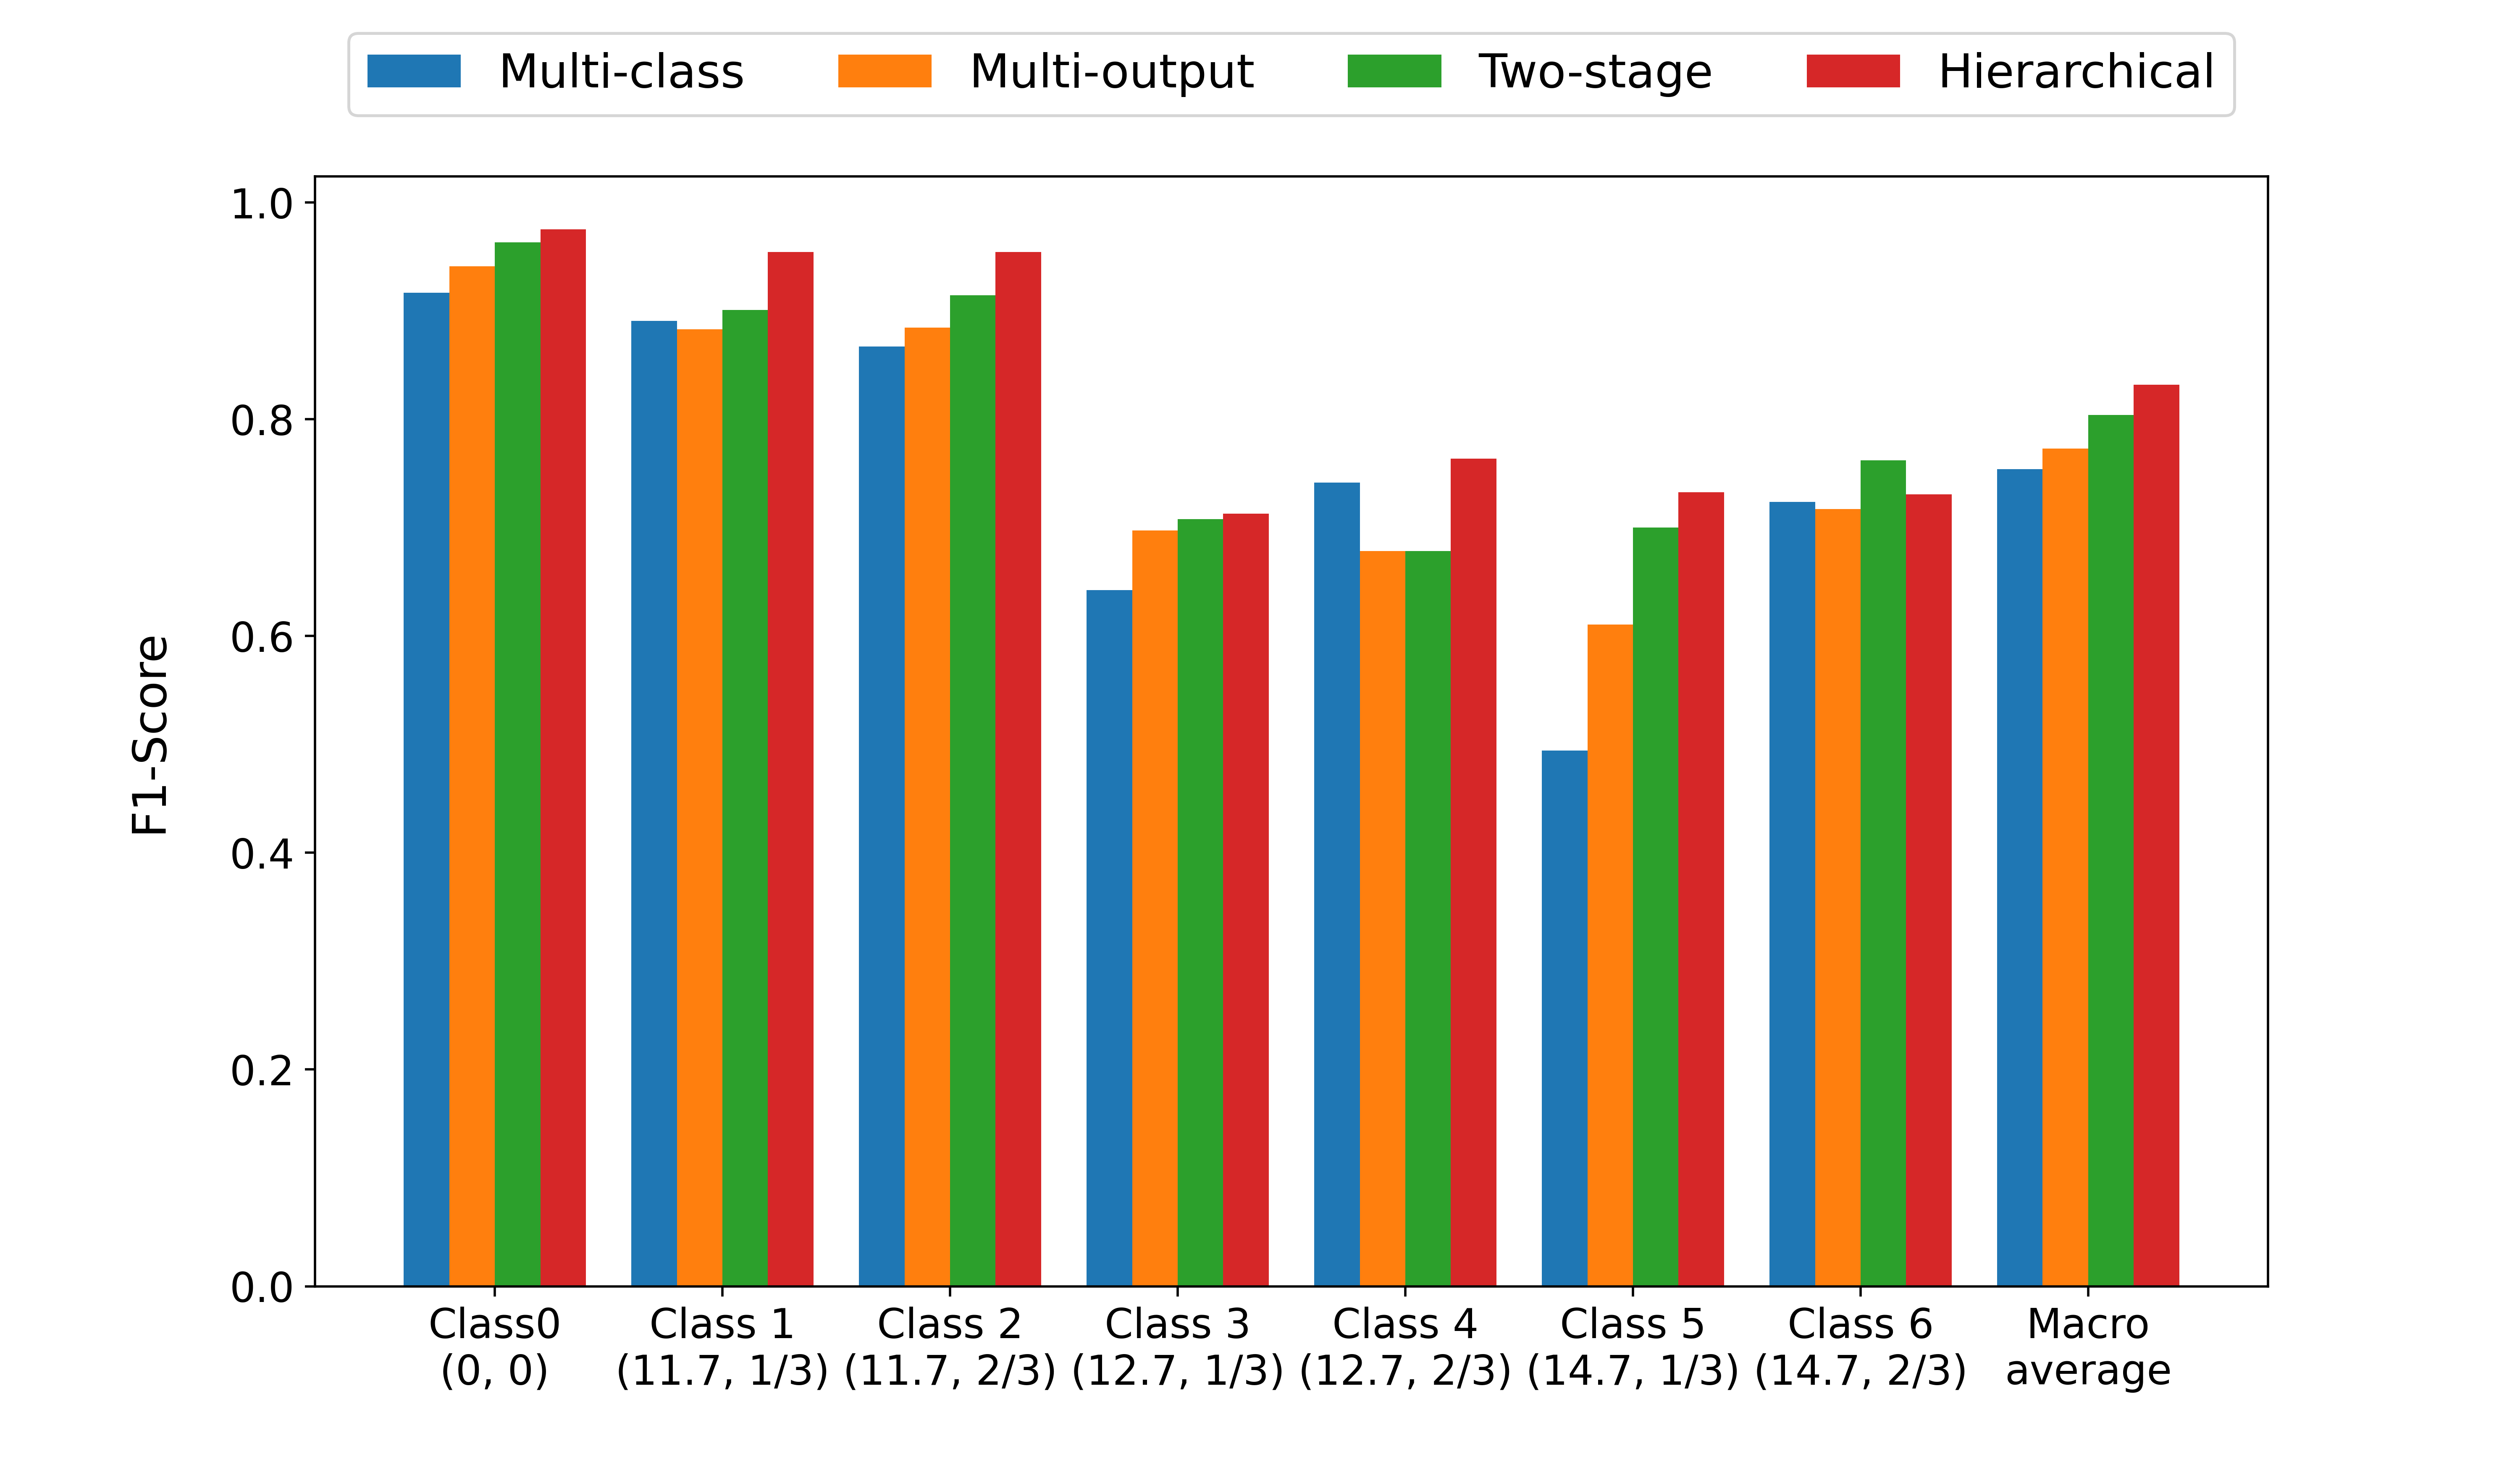
\includegraphics[width=\linewidth]{fig/f1_comparison.png}
    \caption{Comparison of F1-score by class and classifier designs}
    \label{fig: f1 comparison}
\end{figure}

\begin{table}[tb]
    \centering
    \caption{Classification performance of hierarchical classifier}
    \label{table: hier class performance}
    \begin{tabularx}{\textwidth}{
      >{\centering\arraybackslash}X
      >{\centering\arraybackslash\hsize=0.5\hsize}X
      >{\centering\arraybackslash\hsize=0.5\hsize}X
      >{\centering\arraybackslash\hsize=0.5\hsize}X
      >{\centering\arraybackslash\hsize=0.5\hsize}X
    }
    \toprule
    %
    & Precision & Recall & F1-score & No. data \\
    \midrule
    %
    Class 0 \par (0 kN, 0\%) & 0.98 & 1.00 & 0.99 & 81 \\
    %
    Class 1 \par (11.7 kN, 33\%) & 0.96 & 0.96 & 0.96 & 54 \\
    %
    Class 2 \par (11.7 kN, 67\%) & 0.95 & 0.96 & 0.95 & 54 \\
    %
    Class 3 \par (12.7 kN, 33\%) & 0.71 & 0.76 & 0.73 & 54 \\
    %
    Class 4 \par (12.7 kN, 67\%) & 0.74 & 0.80 & 0.77 & 54 \\
    %
    Class 5 \par (14.7 kN, 33\%) & 0.77 & 0.69 & 0.73 & 54 \\
    %
    Class 6 \par (14.7 kN, 67\%) & 0.80 & 0.72 & 0.76 & 54 \\
    \midrule
    %
    Macro Average & 0.84 & 0.84 & 0.84 & 405 \\ 
    %
    Weighted Average & 0.85 & 0.85 & 0.85 & 405 \\ 
    \bottomrule
    \end{tabularx}
\end{table}

\begin{figure}[tb]
    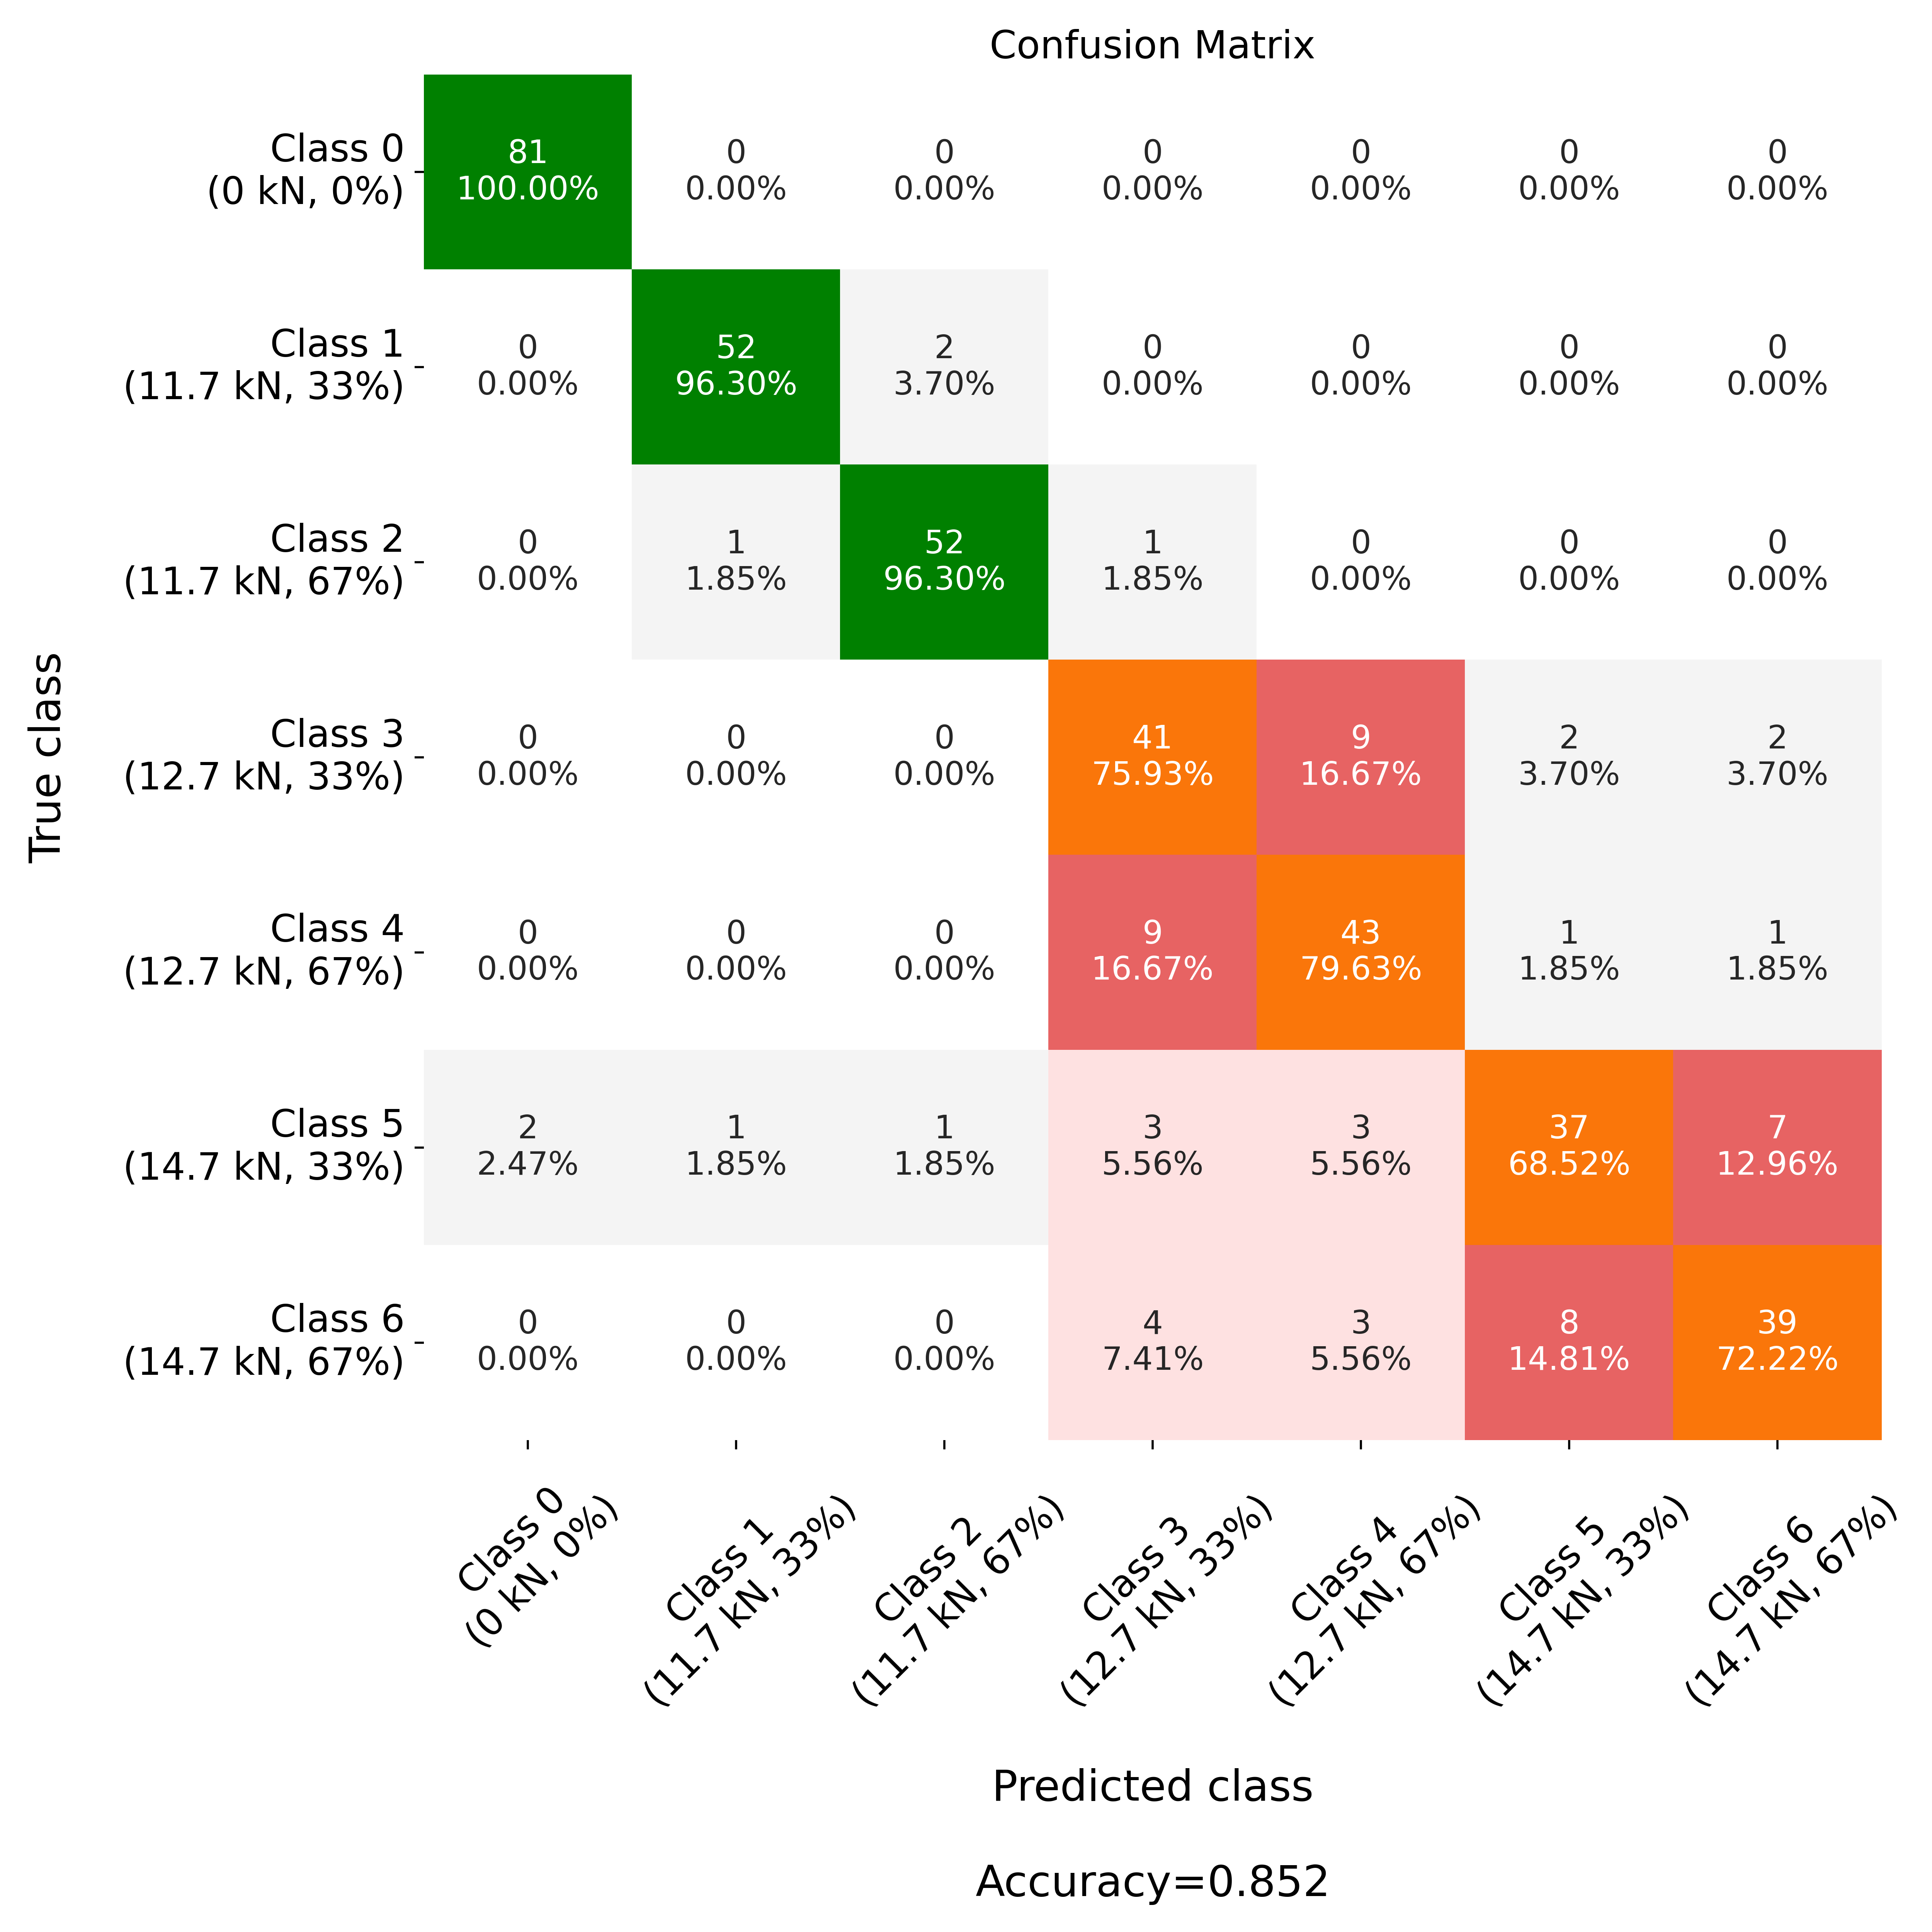
\includegraphics[width=\linewidth]{fig/hierarchical_confusion_matrix.png}
    \caption{Confusion matrix of hierarchical classifier for cross-validation}
    \label{fig: confu mat hier}
\end{figure}


\section{RUL estimation with an S-N curve}
In the proposed framework, after obtaining the predicted loading amplitude and percentage of fatigue life, we estimate the RUL of a sample with the S-N curve of that material.

\subsection{S-N curve with statistical distributions}
\label{subsec: statistical sn curve}
Although an S-N curve is often referred to the best-fit line for fatigue data, fatigue life data can be modeled as statistical distributions to account for the variability in fatigue life. The randomness in fatigue life comes from stochastic behaviors in material fatigue and the variance of microstructure in materials. As a result, the fatigue life has been widely modeled by statistical distributions including Gaussian (normal), log-normal, and Weibull distribution \cite{sn-curve-statistical-model-LI2016}. Due to the limited amount of the available fatigue life data in this research, we use a Gaussian normal distribution to model the fatigue life $X_a$ at a loading amplitude $a$ as
\begin{equation}
    X_a \sim Normal(\hat{\mu_{a}}, \hat{\sigma_{a}}^2)
\end{equation}
where $\hat{\mu_{a}}$ is the sample mean, $\hat{\sigma_{a}}$ is the sample standard deviation at the loading amplitude $a$.

\subsection{RUL inference procedure}
An S-N curve serves as a look-up table for linking a classifier's predictions to RUL. The inference procedure is detailed below:
\begin{enumerate}
    \item Plot the predicted loading amplitude and percentage of fatigue life. For example, the prediction, class 1 (11.7 kN, 33\% fatigue life), is plotted as the red dot in Figure XXX.
    \item Determine the fatigue life with the corresponding loading amplitude from the S-N curve. The fatigue life can be in the format of a single value such as the median fatigue life or a statistical distribution described in Subsection \ref{subsec: statistical sn curve}.
    \item If the fatigue life is represented by a single value, the RUL can be estimated by Equation \eqref{eq: rul - value}: 
    \begin{equation}
        \label{eq: rul - value}
        RUL = N_{fl} - N_{c}
    \end{equation}
    where $N_{fl}$ is the fatigue life from an S-N curve and $N_c$ is the number of cycles translated from the predicted percentage of fatigue life a sample has undergone.

    If the fatigue life at a given loading amplitude is modeled as a normal distribution, the RUL of a sample can be estimated by transforming the fatigue life distribution by a factor of the predicted percentage of fatigue life, as in Equation \eqref{eq: fatigue life dist} to \eqref{eq: rul - dist}:
    \begin{equation}
        \label{eq: fatigue life dist}
        X \sim Normal(\mu, \sigma^2)
    \end{equation}
    \begin{equation}
        \label{eq: rul transform}
        Y = X - pX = (1 - p)X
    \end{equation}
    \begin{equation}
        \label{eq: rul - dist}
        Y \sim Normal((1-p)\mu, (1-p)^2\sigma^2)
    \end{equation}
    where $Y$ is a random variable representing the RUL of a sample; $X$ follows a normal distribution $Normal (\mu, \sigma^2)$ with $\mu$ as the mean and $\sigma^2$ as the variance of the fatigue life, and $F$ is scaled by $p$ which is the predicted percentage of fatigue life. Then, the point estimates, e.g., mean, median, or 25\% quantile, as well as the interval estimate of RUL can be inferred. For instance, the 95\% confidence interval of RUL is
    \begin{equation}
        CI = [(1-p)\mu + z_{0.025} (1-p) \sigma,\ (1-p)\mu + z_{0.975} (1-p) \sigma]
    \end{equation}
\end{enumerate}

\subsection{Examples}
In this subsection, we demonstrate two examples of the RUL estimation based on the proposed framework. Because the true fatigue life of the testing specimens in the interrupted fatigue testing is not available, we cannot calculate the error of the RUL prediction for this stage. Instead, the 95\% confidence intervals of the RUL for specimen 3 and 5 are presented in Table \ref{table: rul 3} and \ref{table: rul 5}. 

In Table \ref{table: rul 3}, the 95\% confidence intervals successfully cover a referencing RUL calculated by subtracting the recorded number of cycles from the mean fatigue life. Among all measurements for specimen 3, only 1 measurement at location 2a is misclassified, indicating the strength of the proposed model in estimating the RUL for samples undergone low-amplitude fatigue cycles. Also, the prediction of the other 2 repeated measurements at location 2a are correct, implying that an accurate decision can be made by considering multiple measurements at one location. For specimen 5 in Table \ref{table: rul 5}, more measurements are misclassified. An interesting observation is, however, shorter RUL is estimated at location 1 and 2, where higher damage levels could happen since the two locations are closer to the center of the specimen. Results for the other specimens are reported in Appendix XX

\begin{sidewaystable}
    
    \caption{RUL estimation for specimen 3}
    \label{table: rul 3}
    \footnotesize{
    \textit{Specimen information} \\
    True label: Class 2 (11.7 kN, 67\% fatigue life) \\
    True number of cycles: 590193 cycles \\
    Fatigue life from S-N curve: 777972 cycles \\
    RUL calculated by true number of cycles: 187779 11.7 kN cycles \\}
    \begin{tabularx}{\textwidth}{*{10}{
        >{\centering\arraybackslash}X}
      }
      \toprule
      %
      & \multicolumn{9}{c}{Measurement Location} \\
      \cmidrule(lr){2-10}
      Replicate & 5a & 4a & 3a & 2a & 1 & 2 & 3 & 4 & 5 \\
      \midrule
      %
      1 & [132439, 386208] 11.7 kN \par (2) & [132439, 386208] 11.7 kN \par (2) & [132439, 386208] 11.7 kN \par (2) & [132439, 386208] 11.7 kN \par (2) & [132439, 386208] 11.7 kN \par (2) & [132439, 386208] 11.7 kN \par (2) & [132439, 386208] 11.7 kN \par (2) & [132439, 386208] 11.7 kN \par (2) & [132439, 386208] 11.7 kN \par (2) \\
      2 & [132439, 386208] 11.7 kN \par (2) & [132439, 386208] 11.7 kN \par (2) & [132439, 386208] 11.7 kN \par (2) & [132439, 386208] 11.7 kN \par (2) & [132439, 386208] 11.7 kN \par (2) & [132439, 386208] 11.7 kN \par (2) & [132439, 386208] 11.7 kN \par (2) & [132439, 386208] 11.7 kN \par (2) & [132439, 386208] 11.7 kN \par (2) \\
      3 & [132439, 386208] 11.7 kN \par (2) & [132439, 386208] 11.7 kN \par (2) & [132439, 386208] 11.7 kN \par (2) & \textbf{[264878, 772417] 11.7 kN (1)} & [132439, 386208] 11.7 kN \par (2) & [132439, 386208] 11.7 kN \par (2) & [132439, 386208] 11.7 kN \par (2) & [132439, 386208] 11.7 kN \par (2) & [[132439, 386208] 11.7 kN \par (2) \\
      \bottomrule
    \end{tabularx}
    \footnotesize{95\% confidence interval in square brackets\\
    Predicted class in parentheses\\
    Bold text indicates misclassified measurements}
    
\end{sidewaystable}

\begin{sidewaystable}
    
    \caption{RUL estimation for specimen 5}
    \label{table: rul 5}
    \footnotesize{
    \textit{Specimen information} \\
    True label: Class 3 (12.7 kN, 33\% fatigue life) \\
    True number of cycles: 90011 cycles \\
    Fatigue life from S-N curve: 342110 cycles \\
    RUL calculated by true number of cycles: 252099 12.7 kN cycles \\}
    \begin{tabularx}{\textwidth}{*{10}{
        >{\centering\arraybackslash}X}
      }
      \toprule
      %
      & \multicolumn{9}{c}{Measurement Location} \\
      \cmidrule(lr){2-10}
      Replicate & 5a & 4a & 3a & 2a & 1 & 2 & 3 & 4 & 5 \\
      \midrule
      %
      1 & [117963, 338183] 12.7 kN \par (3) & [117963, 338183] 12.7 kN \par (3) & [117963, 338183] 12.7 kN (3) & [117963, 338183] 12.7 kN \par (3) & \textbf{[58981, 169091] 12.7kN (4)} & \textbf{[58981, 169091] 12.7kN (4)} & [117963, 338183] 12.7 kN \par (3) & [117963, 338183] 12.7 kN \par (3) & [117963, 338183] 12.7 kN \\
      2 & \textbf{[58981, 169091] 12.7kN (4)} & [117963, 338183] 12.7 kN \par (3) & [117963, 338183] 12.7 kN \par (3) & [117963, 338183] 12.7 kN \par (3) & \textbf{[58981, 169091] 12.7kN (4)} & \textbf{[58981, 169091] 12.7kN (4)} & \textbf{[18754, 49107] 14.7kN (6)} & [117963, 338183] 12.7 kN \par (3) & [117963, 338183] 12.7 kN \par (3) \\
      3 & [117963, 338183] 12.7 kN \par (3) & \textbf{[58981, 169091] 12.7kN (4)} & [117963, 338183] 12.7 kN \par (3) & [117963, 338183] 12.7 kN \par (3) & \textbf{\textbf{[58981, 169091] 12.7kN (4)}} & [117963, 338183] 12.7 kN \par (3) & [117963, 338183] 12.7 kN \par (3) & [117963, 338183] 12.7 kN \par (3) & [117963, 338183] 12.7 kN \par (3) \\
      \bottomrule
    \end{tabularx}
    \footnotesize{95\% confidence interval in square brackets\\
    Predicted class in parentheses\\
    Bold text indicates misclassified measurements}
    
\end{sidewaystable}


\section{Discussion}
This section discusses several findings and limitations of the RUL prediction framework including 
\begin{enumerate*}[label=\itshape\alph*\upshape)]
    \item impacts of classifier designs and the structure of data, and
    \item Decision making based on multiple measurements.
\end{enumerate*}
Other take ways and issues are mentioned in Chapter \ref{chap: concl}.

\subsection{impacts of classifier designs and the structure of data}
As presented in Section \ref{sec: design of classifiers}, a major problem can be decomposed into several sub-tasks by adopting a divide-and-conquer manner and the error rates can be reduced. In Table \ref{table: summary class algo}, one can observe that the prediction accuracy increases from 77.3\% (multi-class classifier) to 85.3\% (hierarchical classifier) as we split the meta classification problem into smaller classification tasks by exploiting the structure of the data. Nevertheless, the caveat is that introducing more classifiers for subtasks can increase the risk of overfitting the small dataset. The trade off between the generalizability and the performance of a model and other classifier designs are left for further investigation.

\subsection{Decision making based on multiple measurements}
In the design of experiments, the ultrasonic measurements were conducted at different locations across the specimen and at one location repeatedly, offering opportunities for practitioners to make decision based on the information from the spatial and repeated measurements. For example, one can determine the RUL of a specimen by selecting the minimum, average, or mode RUL among the three repeated measurements at one location. Furthermore, the RUL of an entire specimen can be evaluated by similar or even more sophisticated approaches across multiple locations to decide the usability of a component. These rules are worth investigating in the real application scenarios.
